\section{Evaluation}
\label{sec:evaluation}

All the results presented in this section are obtained with the following parameters:
\begin{itemize}
    \item $n_D = 50$
    \item $n_{max} = 250$
    \item $N = 200$
\end{itemize}

\subsection{Minover}
\begin{figure}[t]
	\centering
	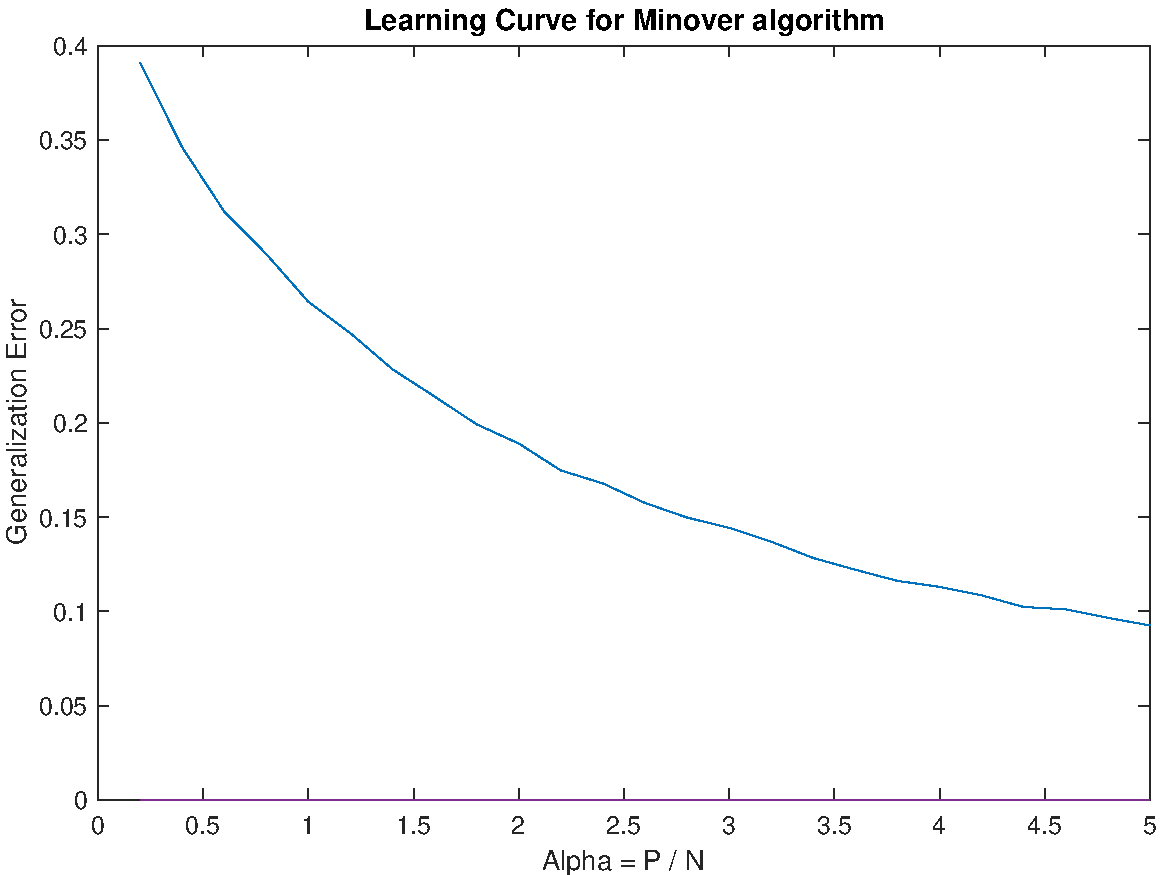
\includegraphics[width=\columnwidth]{figures/base}
    \caption{Generalization error of a perceptron trained with the Minover algorithm on a linearly separable dataset.}
	\label{fig:base}
\end{figure}

\cref{fig:base} shows the generalization error of the perceptron trained with the Minover algorithm on a linearly separable dataset (with no noise, $\lambda = 0$).
Since the number of dimensions of the dataset $N$ is fixed, $\alpha = P / N$ is proportional to the number of examples $P$ used for the training.
The generalization error decreases for higher values of $\alpha$, i.e. when the number of examples increases.
In other words, it seems to be the case:
$$\lim_{P \to \infty} w = w^{*}$$

The examples are distributed in all the space and the boundary between the classes is fixed and determined by the teacher vector $w^{*}$.
Intuitively, for an higher number of examples $P$, the maximum margin between the $2$ classes, since it is more likely that some example is really close to the boundary hyperplane determined by $w^{*}$.
Since the Minover algorithm tries to find some separation hyperplane, it is easier to get closer to the teacher vector $w^{*}$ if the maximum possible margin is smaller.


\subsection{Minover vs Rosenblatt}
\begin{figure}[t]
	\centering
	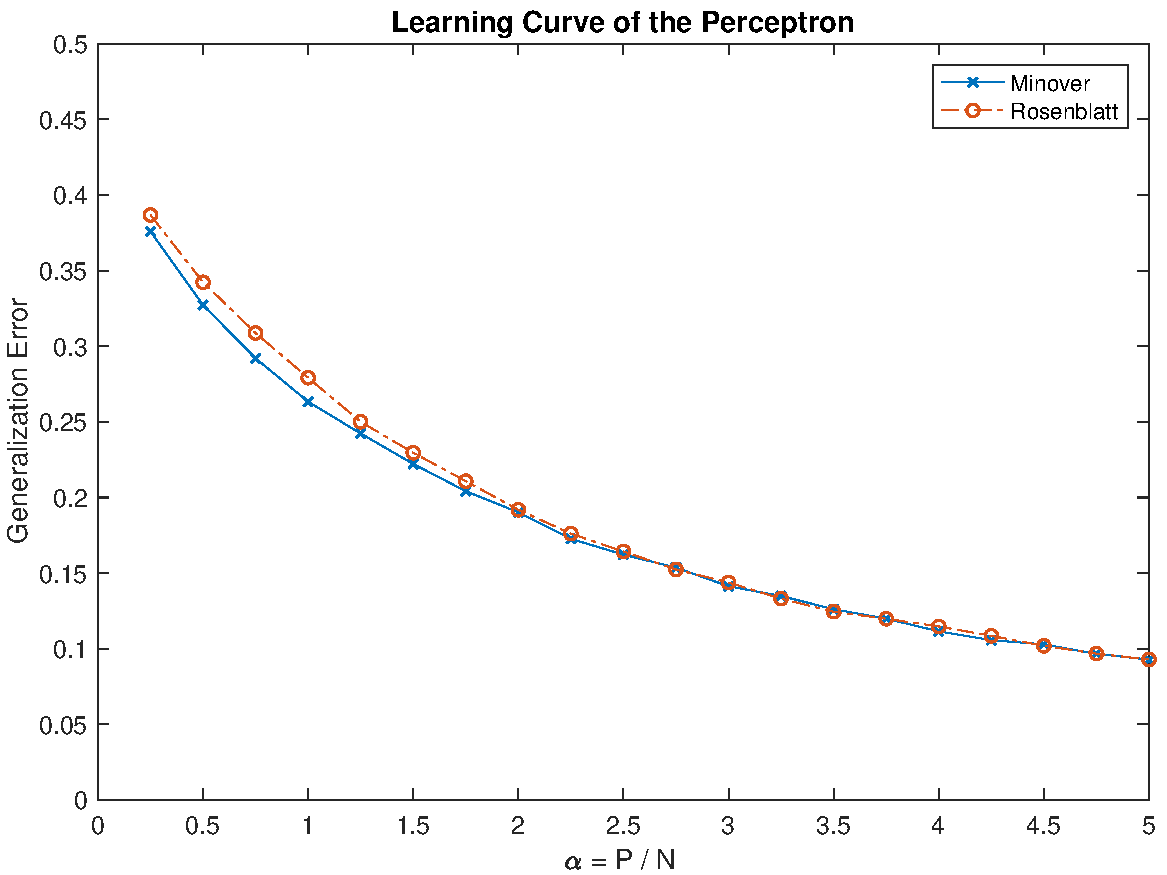
\includegraphics[width=\columnwidth]{figures/comparison}
    \caption{Generalization error for the Minover and the Rosenblatt algorithms on a linearly separable dataset.}
	\label{fig:comparison}
\end{figure}

\cref{fig:base} shows the generalization error of the perceptron trained with the Minover and the Rosenblatt algorithms on a linearly separable dataset (with no noise, $\lambda = 0$).
For both algorithms the generalization error decreases with higher numbers of examples for the training (see the previous section).
In absence of noise, the performances of the $2$ algorithms are quite close, with Minover performing slightly better than Rosenblatt for low values of $\alpha$.


\subsection{Noise}
